% AI-assisted working draft for team review, not an approved final section.
% Requires amsmath, graphicx and booktabs. Merge references.bib into the report bibliography.
\section{Additional objects and experimental design}
\label{sec:objects}

The square of Section~\ref{sec:square} is stretched almost uniformly, has
an exact check and uses a structured mesh. Openings, corners, slender
members and other supports raise new questions: how shape concentrates
deformation and stress, whether geometry and supports change the
conditioning of $A$ and hence solver cost, and whether findings on
structured meshes carry over to general triangulations. We specify four
objects and comparisons that change one factor at a time;
Section~\ref{sec:results} reports the outcomes.

\subsection{Objects and meshes}
Table~\ref{tab:objects-objects} and Fig.~\ref{fig:objects-meshes} define
the objects; all four are selected experiments, not illustrations. The
square \textsf{S} repeats Section~\ref{sec:square} on an unstructured mesh.
The plate \textsf{H} adds a central hole, the classical stress raiser: in a
wide plate under tension the stress at a small hole is three times the
applied value~\cite{timoshenko-goodier}. The bracket \textsf{L} has a
re-entrant corner, where the continuum stress is
unbounded~\cite{williams-corners}, so local stresses there cannot converge
under refinement; its two free arm ends let the load move while $A$ stays
fixed. The beam \textsf{B} bends under a tip load, which beam theory
predicts and linear triangles represent poorly on coarse
meshes~\cite{cook-fea}.

\begin{table}[htbp]
 \centering
 \caption{Objects, with ordered counter-clockwise outer vertices. All are
 clamped on $x=0$. $N$: unknowns on mesh levels 1--4.}
 \label{tab:objects-objects}
 \footnotesize\setlength{\tabcolsep}{4pt}
 \begin{tabular}{@{}lllll@{}}
 \toprule
 Object & Outer boundary (m) & Opening & Load & $N$, levels 1--4 \\
 \midrule
 \textsf{S} square & $(0,0),(1,0),(1,1),(0,1)$ & -- & $(p,0)$, $x=1$ & 390/1484/3350/5936 \\
 \textsf{H} plate & as \textsf{S} & disc $(0.5,0.5)$, $R=0.15$ & $(p,0)$, $x=1$ & 380/1414/3150/5564 \\
 \textsf{L} bracket & $(0,0),(1,0),(1,\frac12),(\frac12,\frac12),(\frac12,1),(0,1)$ & -- & $(p,0)$, $x=1$ & 302/1132/2498/4470 \\
 \textsf{B} beam & $(0,0),(4,0),(4,0.5),(0,0.5)$ & -- & $(0,-\tau)$, $x=4$ & 534/2020/4414/7776 \\
 \bottomrule
 \end{tabular}
\end{table}

Boundary segments are labelled clamped, loaded or free and split into
equal pieces of length at most $h$. Triangle~\cite{shewchuk-triangle},
through its Python interface~\cite{rufat-triangle}, then builds a
constrained Delaunay mesh with switches \texttt{p} (keep segments),
\texttt{q30} (angles at least $30^\circ$) and \texttt{a} (area at most
$\sqrt3h^2/4$, an equilateral triangle of side $h$); subsegments inherit
the labels. The hole is an inscribed regular polygon with
$4\lceil2\pi R/(4h)\rceil$ vertices and a seed point from which Triangle
removes all triangles. Matched points (Fig.~\ref{fig:objects-meshes}) are
input vertices, hence nodes on every level. The levels use $h=0.1$, $0.05$,
$1/30$ and $0.025$~m, and $h=0.125$, $0.0625$, $1/24$ and $0.03125$~m for
\textsf{B} (4 to 16 elements through its depth). Every mesh passes these
checks: positive counter-clockwise areas summing to the polygon area,
boundary edges equal to the labelled subsegments, no triangle in the hole,
and one connected piece with Euler characteristic $1$ minus the number of
holes. The polygon's small area difference from the disc vanishes as
$h\to0$ and is part of the discretization error.

\begin{figure}[htbp]
 \centering
 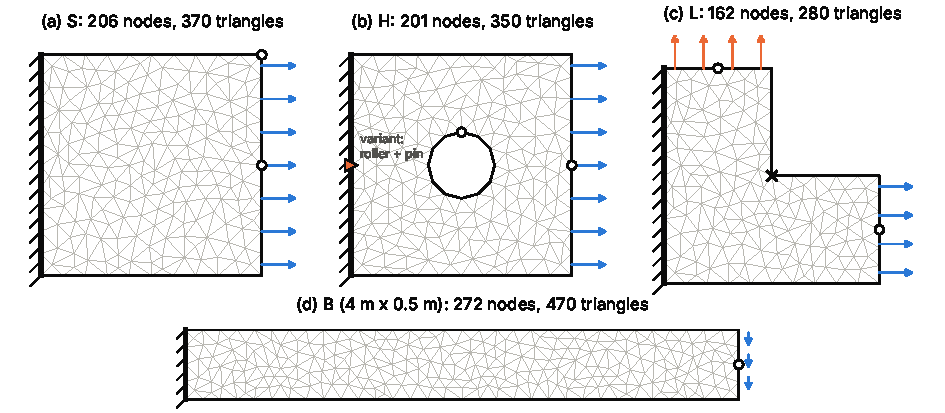
\includegraphics[width=0.92\linewidth]{figures/objects_meshes.pdf}
 \caption{The objects on their level-1 meshes. Hatching: clamped edge.
 Blue arrows: baseline traction. Dashed orange arrows: alternative load on
 \textsf{L}. Orange triangle: pin of the roller variant of \textsf{H}.
 Circles: matched points; cross: re-entrant corner.}
 \label{fig:objects-meshes}
\end{figure}

\subsection{Material, loads and supports}
Material, thickness, plane stress and the clamp follow
Section~\ref{sec:square}. \textsf{S}, \textsf{H} and \textsf{L} carry the
normal traction $p=100$~MPa on their face $x=1$, with resultant $10^6$~N,
or $5\times10^5$~N for \textsf{L}. The beam, of length $L_B=4$~m and depth
$W_B=0.5$~m, carries the downward tip traction $\tau=10$~MPa, so
$P=\tau tW_B=5\times10^4$~N and strains stay of order $10^{-3}$. Beam
theory gives the tip deflection~\cite{timoshenko-goodier}
\begin{equation}
 \delta\approx\frac{PL_B^3}{3EI}+\frac{PL_B}{\kappa_sGtW_B},\qquad
 I=\frac{tW_B^3}{12},\quad G=\frac{E}{2(1+\nu)},\quad\kappa_s=\frac56,
 \label{eq:objects-beam}
\end{equation}
that is, 51.20~mm from bending plus 0.62~mm from shear; our clamp also
prevents warping of the root section, which beam theory ignores.

Loads enter as consistent nodal forces, $\ell_eq/2$ at each end of a loaded
edge of length $\ell_e$ (Section~\ref{sec:mechanics-matrix}). Because loads
and clamps are tied to labelled segments, every level carries the same
resultant on the same face and is held on the same edge. A clamped edge
removes both translations and the rotation. We confirm that every reduced
$A$ is positive definite through a positive smallest eigenvalue
(shift-invert \texttt{eigsh}) and, up to 3000 unknowns, a dense Cholesky
factorization. As a negative control, restraining only $u_x$ on $x=0$
leaves a vertical translation that this check must flag.

\subsection{Case register}
Table~\ref{tab:objects-register} lists the comparisons. The geometry study
fixes support, traction and mesh rule, so differences come from shape. The
refinement study estimates discretization error from changes at matched
points, tests whether $\kappa_2$ grows like $h^{-2}$ and CG iterations like
$\sqrt{\kappa_2}$ (Section~\ref{sec:solvers}), and uses peak element
stresses to show where local quantities converge. On unstructured meshes
the diagonal of $A$ varies with element shape, which
Section~\ref{sec:solvers} names as the condition for diagonal
preconditioning to help; the mesh-type study compares this with the grids
of Section~\ref{sec:square}.

\begin{table}[htbp]
 \centering
 \caption{Case register. Variants of \textsf{H}, \textsf{L} and \textsf{B}
 use level 2. $u_P$: displacement at a matched point.}
 \label{tab:objects-register}
 \footnotesize\setlength{\tabcolsep}{4pt}
 \begin{tabular}{@{}lllll@{}}
 \toprule
 Study & Question & Changed factor & Fixed & Measured response \\
 \midrule
 Geometry & shape effect & \textsf{S}, \textsf{H}, \textsf{L} & load, clamp, $h$ & $u_P$, $\kappa_2$, iterations \\
 Refinement & convergence, cost & $h$, levels 1--4 & object, load, supports & $u_P$, peak stress, $\kappa_2$, $\rho_J$, iterations \\
 Mesh type & structured vs Triangle & grid, $n=10$--40, vs \textsf{S} & square problem & $u_P$, $\kappa_2$, CG/PCG iterations \\
 Load size & linearity & $p=25$, 100, 250~MPa (\textsf{H}) & $A$ & $u_P/p$, iterations \\
 Load location & load position & face $x=1$ vs $y=1$ (\textsf{L}) & $A$, resultant & loaded-face $u_P$, iterations \\
 Supports & clamp vs roller+pin & $u_x=0$ on $x=0$, $u_y=0$ at $(0,\frac12)$ (\textsf{H}) & load, mesh & $u_P$, $\kappa_2$, iterations \\
 Material & role of $E$, $\nu$ & $\nu=0$, 0.3, 0.45; $E=70$, 200~GPa (\textsf{H}) & geometry, load & $u_P$, $\kappa_2$, iterations \\
 Bending & bending accuracy & $h$, levels 1--4 (\textsf{B}) & beam, $P$ & tip $u_y$ vs Eq.~\eqref{eq:objects-beam}, $\kappa_2$ \\
 Load type & axial vs bending & $(p,0)$ vs $(0,-\tau)$ on tip (\textsf{B}) & $A$ & tip $u_x$ vs $pL_B/E$, iterations \\
 \bottomrule
 \end{tabular}
\end{table}

Several studies have known answers that test the implementation. Scaling
$p$ scales $b$ and $x$ but not the iteration counts, since $\eta$ is scale
invariant. Scaling $E$ scales $A$, so $x\propto1/E$ while $\kappa_2$ is
unchanged. The two bracket loads, and the two beam loads, share $A$, which
isolates the right-hand side. Changing $\nu$ or the supports changes $A$
itself.

Every reduced system is solved by sparse LU, CG, diagonal PCG, MINRES and
Gauss--Seidel under the protocol of Section~\ref{sec:solvers}; each
level-2 baseline also receives all eight iterative methods. A capped
Gauss--Seidel run takes tens of seconds, so it is timed once, without a
history run, except on levels 1--2 of the baselines. Each solution is
validated by the force and moment balance of loads and reactions,
Eq.~\eqref{eq:mechanics-reactions}, and by $d_C=0$. All outputs come from
\texttt{draft/experiments/objects.py}.
